\documentclass[12pt]{article}
\usepackage{geometry}                % See geometry.pdf to learn the layout options. There are lots.
\geometry{letterpaper}                   % ... or a4paper or a5paper or ... 
%\geometry{landscape}                % Activate for for rotated page geometry
\usepackage[parfill]{parskip}    % Activate to begin paragraphs with an empty line rather than an indent
\usepackage{daves,fancyhdr,natbib,graphicx,dcolumn,amsmath,lastpage,url}
\usepackage{amsmath,amssymb,epstopdf,longtable}
\usepackage{paralist}  % need to properly formulate standard answer blocks
\usepackage[final]{pdfpages}
\DeclareGraphicsRule{.tif}{png}{.png}{`convert #1 `dirname #1`/`basename #1 .tif`.png}
\pagestyle{fancy}
\lhead{CE 3305 Fluid Mechanics; Exercise Set 15}
\rhead{Name:\_\_\_\_\_\_\_\_\_\_\_\_\_\_\_\_\_\_\_\_\_\_\_\_\_\_\_\_\_\_\_\_\_\_}
\lfoot{REVISION A}
\cfoot{}
\rfoot{Page \thepage\ of \pageref{LastPage}}
\renewcommand\headrulewidth{0pt}
%%%%%%%%%%%%%%%%%%%%%%%%%%%%%%%%%%%%
\begin{document}
%%%%%%%%%%%%%%%%%%%%%%%%%%%%%%%%%%%
\begingroup
\begin{center}
{\textbf{{ CE 3305 Engineering Fluid Mechanics} \\ Exercise Set 15 \\ Summer 2018 -- GERMANY} }
\end{center}
\endgroup
\begingroup
~\newline
\textbf{Purpose} :  Modified Bernoulli's Equation (Head Losses) in hydraulics systems \\
\textbf{Assessment Criteria} : Completion, plausible solutions, use \textbf{R} as a calculator. \\~\\
\textbf{Exercises}

\begin{enumerate}
\item (Problem 7.34 pg 283)  Figure \ref{fig:TankDrainb} depicts a reservoir draining through a valve used to control the flow rate.
The head loss across the valve is $h_l = \frac{4V^2}{2g}$, where $V$ is the velocity in the pipe.
The cross-sectional area of the pipe is 8 $cm^2$.
All loss occurs in the valve.
The elevation of the water level in the reservoir above the pipe outlet is 9 $m$.
Find the discharge in the pipe; assume $\alpha = 1.0$ at all locations in the system.
\begin{figure}[h!] %  figure placement: here, top, bottom, or page
   \centering
   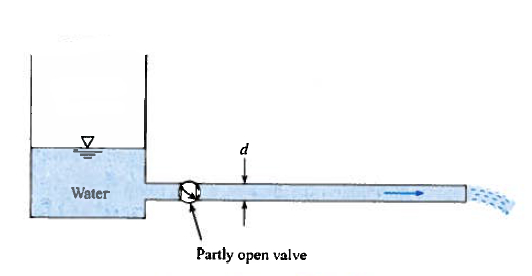
\includegraphics[width=2.8in]{TankDrainb.jpg} 
   \caption{Reservoir draining through a valve and a pipe}
   \label{fig:TankDrainb}
\end{figure}
\item (Problem 7.48 pg 285) Figure \ref{fig:PumpLoss} is a schematic of a pump system that supplies water to a hydraulic component through a 15 $cm$ diameter, 60 $m$ length of pipe.
The mean velocity in the pipe is 2 $m/s$, and the head loss in the pipe is 2 $m$.   
Determine the pressure drop in the horizontal pipe and the power required from the pump to overcome the head loss in the pipe.
\begin{figure}[h!] %  figure placement: here, top, bottom, or page
   \centering
   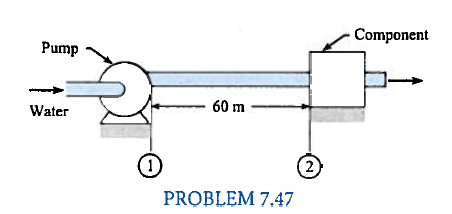
\includegraphics[width=2.8in]{PumpLoss.jpg} 
   \caption{Pumping system}
   \label{fig:PumpLoss}
\end{figure}

\end{enumerate}
\end{document}  